%%%%%%%%%%%%%%%%%%%%%%%%%%%%%%%%%%%%%%%%%%%%%%
%                insertmeeting
% 1) Title (something creative & funny?)
% 2) Date (MM/DD/YYYY)
% 3) Location (ex. Hagerty High School)
% 4) People/Committees Present 
% 5) Picture 
% 6) Start Time & Stop Time (ex. 12:30AM to 4:30PM)
%%%%%%%%%%%%%%%%%%%%%%%%%%%%%%%%%%%%%%%%%%%%%%
\insertmeeting 
	{CAD Cataclysm} 
	{08/08/21}
	{Hagerty High School}
	{Nathan}
	{Images/RobotPics/robot.jpg}
	{4:00 - 5:40}
	
\subsection*{Hardware}
\noindent\hfil\rule{\textwidth}{.4pt}\hfil
\subsubsection*{Goals}
\begin{itemize}
    \item Come up with a way to organize electronics
    \item Design rev hub and battery holder in onshape
  

\end{itemize} 

\noindent\hfil\rule{\textwidth}{.4pt}\hfil

\subsubsection*{Accomplishments}
 In previous years, we have waited too long to test our mechanisms because our electronics weren’t set up or unorganized - this wasted valueable time and got in the way. To get ahead we decided to make a rev hub and battery holder in order to be able to start the season with a working (easily assembled drivetrain.)
To design the holder we found and downloaded step files of the rev hubs and batteries we will be using in the upcoming season to act as a size reference. Once finding these files we discussed several different arrangements for the rev hubs and battery. After brainstorming several different options, considering both compactness and accessibility, we chose to have a two-tiered tray. The smaller, lower level would hold the battery while the more accessible upper level would hold the two rev hubs.
We started designing the parts for this assembly in CAD with flexibility in mind. Because the game hasn’t been announced yet, we know that we will likely need to change some major aspects of the design. With this in mind, we ensured that the major features of the cad were constrained to features on the drive plates, like the churros, so that if we change the skeleton for the drive plates, everything else will change around it. It was easy to base features of this design on that of the drive plate because we created all of the parts in the same part studio as the drive plates. This means that we can just project features from the drive plate skeleton directly. We already knew that we wanted to support all of these parts on the churros, so we started by creating vertical connectors between the churros and the plates that will support the rev hubs and battery. (image 1 and image 2) After making this plate we created the horizontal plates that hold the electronics, connecting the plates to the vertical connectors using box joints and t-slot joints.
Once we had made all of these parts, we brought them into the drivetrain assembly to ensure that the pieces all fit together properly (image 3). One thing that we forgot to account for was the middle odometer. Because we are hoping to use odometry for the first time this year, we aren’t used to accounting for the extra space needed, so we had forgotten to add a spot for the odometers. Luckily, we left a spot open in the center where we could easily add another plate to attach the odometer. (Image 4)After adding this plate and some extra supports, we had completed all of the necessary parts to this design, but we wanted to test out an additional design for a 3d printed part that could clip to the churro and hold any plate we attach to it in the same place without sliding (Image 5). Although it wouldn’t be particularly helpful for this part of the robot, this is a good opportunity to test the clamp part out because if it doesn’t work properly, we can still continue building the rest of the rev hub assembly without needing to redesign immediately. After adding all of the new parts in the assembly, we had completed the design (Image 6).

\begin{figure}[htp]
\centering
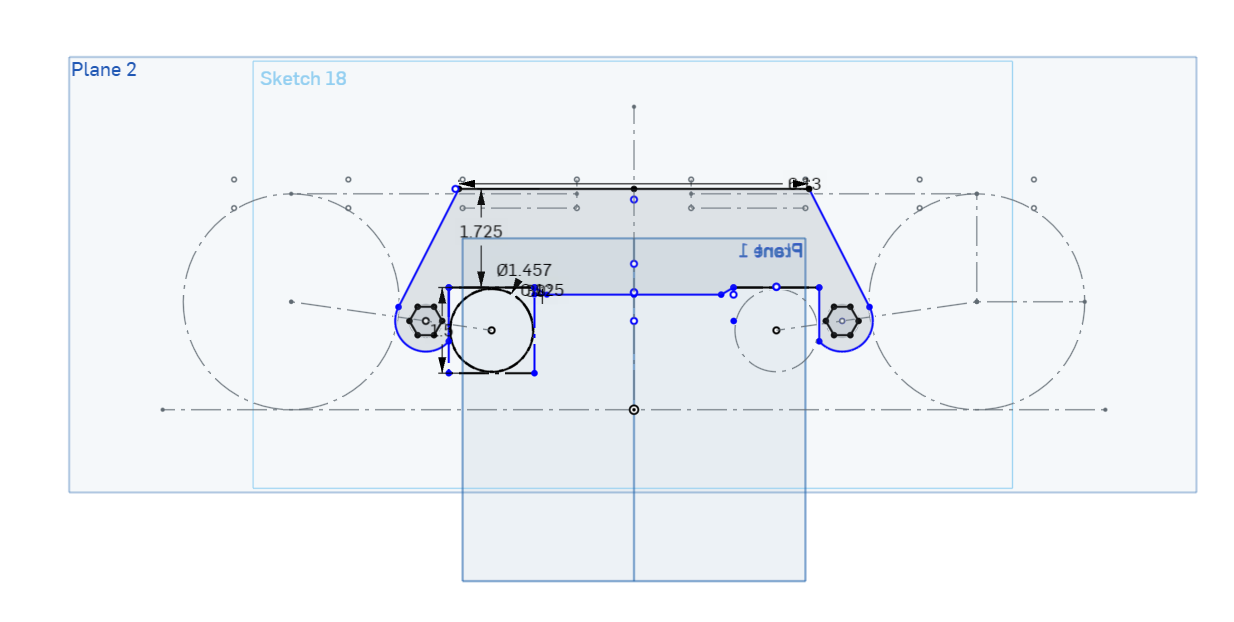
\includegraphics[width=0.9\textwidth, angle=0]{Meetings/August/08-08-21/8-8-21_Image1-SupportSketch - Nathan Forrer.PNG}
\caption{The support sketch for the initial drivetrain plate.}
\label{fig:pic1}
\end{figure}

\begin{figure}[htp]
\centering
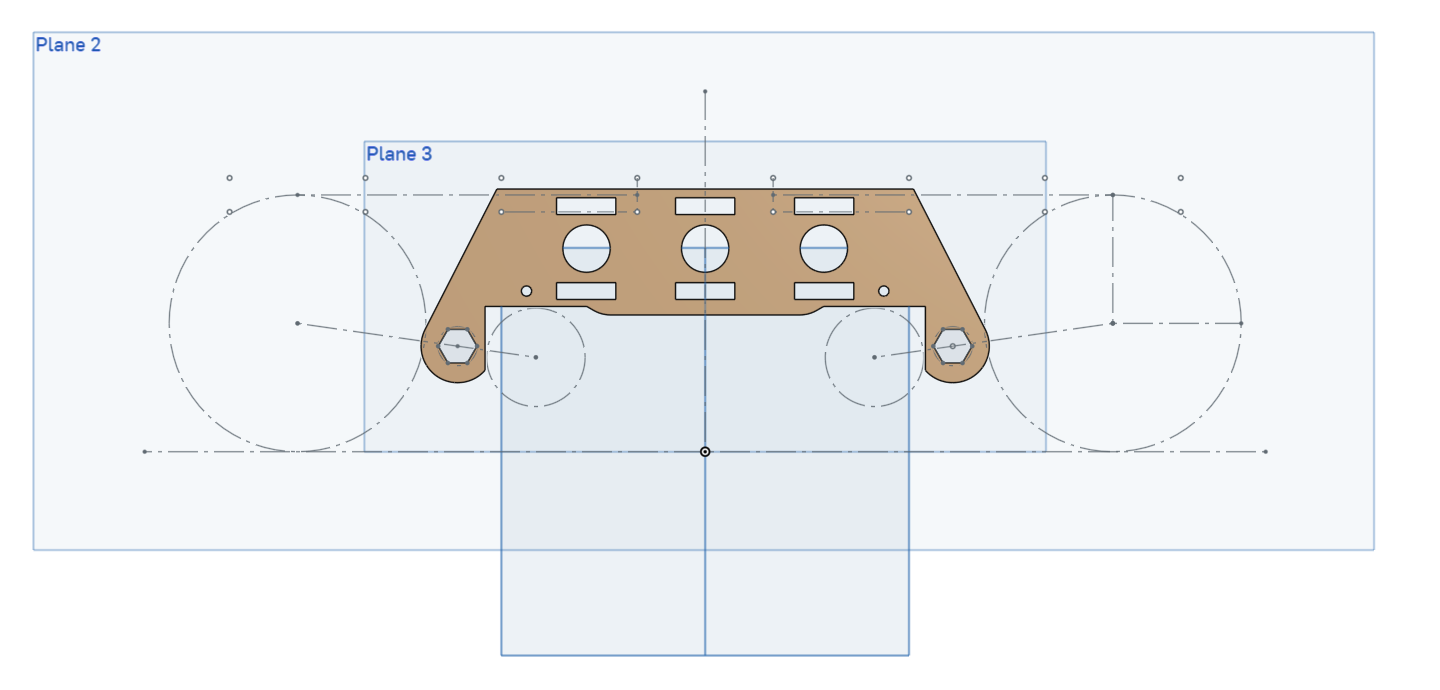
\includegraphics[width=0.9\textwidth, angle=0]{Meetings/August/08-08-21/8-8-21_Image2-SupportPart - Nathan Forrer.PNG}
\caption{The extruded part for the initial drivetrain plate using the support sketch.}
\label{fig:pic2}
\end{figure}

\begin{figure}[htp]
\centering
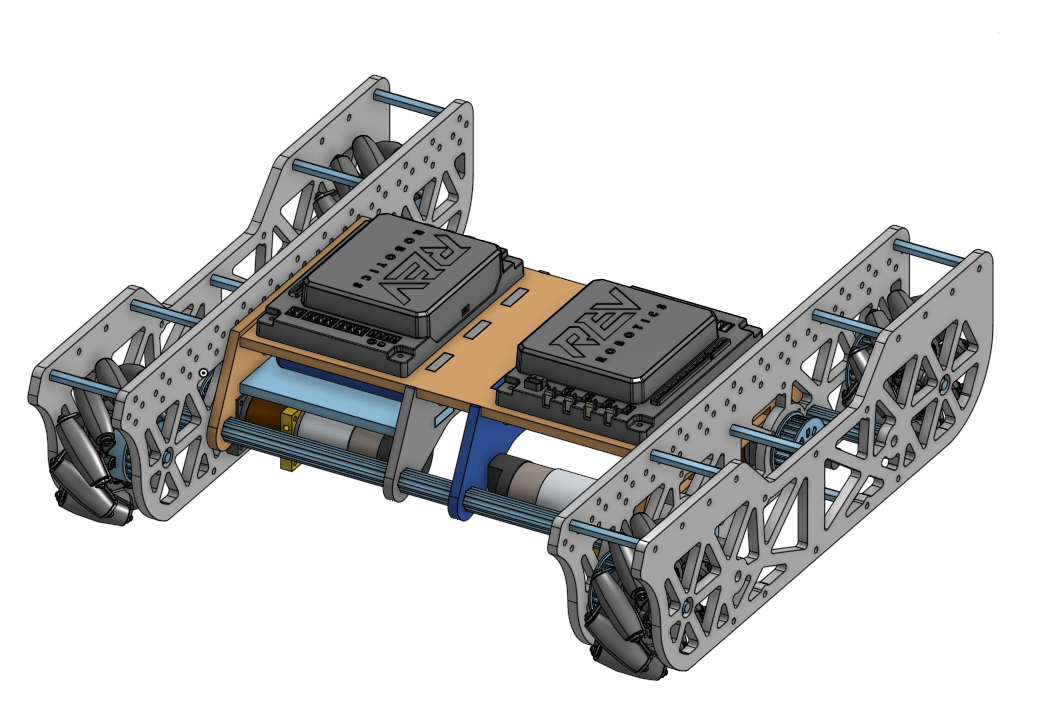
\includegraphics[width=0.9\textwidth, angle=0]{Meetings/August/08-08-21/8-8-21_Image3-Assembly1 - Nathan Forrer.PNG}
\caption{The full assembly for our mecanum drivetrain.}
\label{fig:pic3}
\end{figure}

\begin{figure}[htp]
\centering
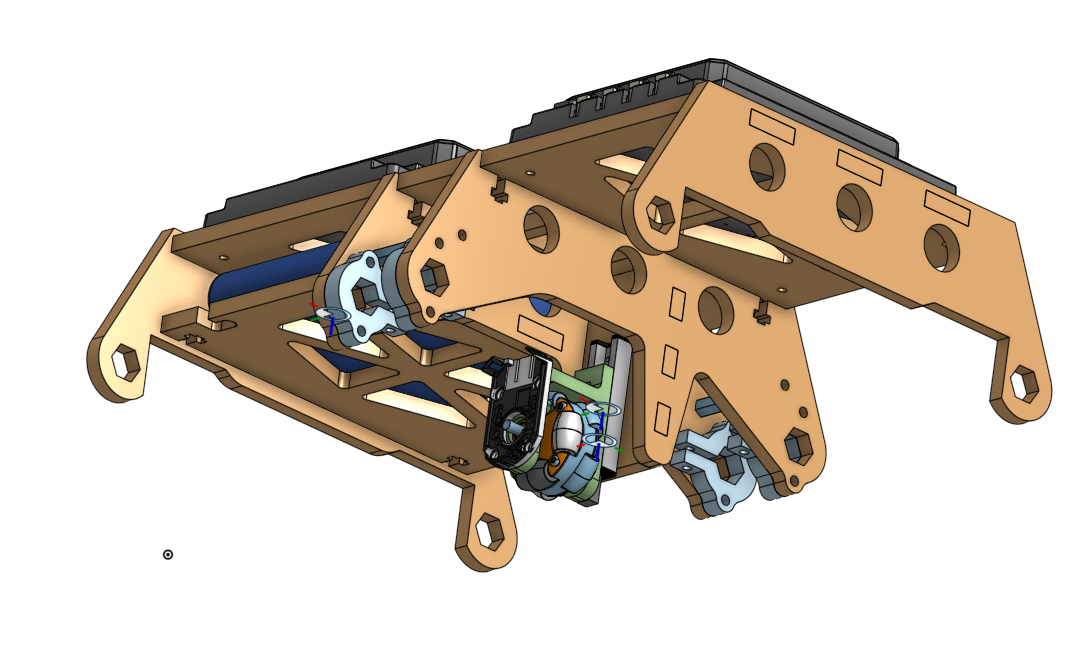
\includegraphics[width=0.9\textwidth, angle=0]{Meetings/August/08-08-21/8-8-21_Image4-Odometer - Nathan Forrer.PNG}
\caption{Our odometer is shown in the middle of the assembly. We plan to use this to aid our robot localization.}
\label{fig:pic4}
\end{figure}

\begin{figure}[htp]
\centering
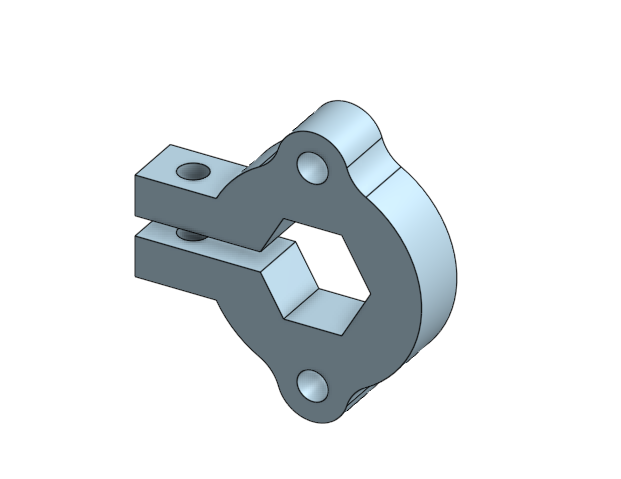
\includegraphics[width=0.9\textwidth, angle=0]{Meetings/August/08-08-21/8-8-21_Image5-Clip - Nathan Forrer.PNG}
\caption{The final CAD design for the clip we are using to secure the churros passing through the drivetrain.}
\label{fig:pic5}
\end{figure}

\begin{figure}[htp]
\centering
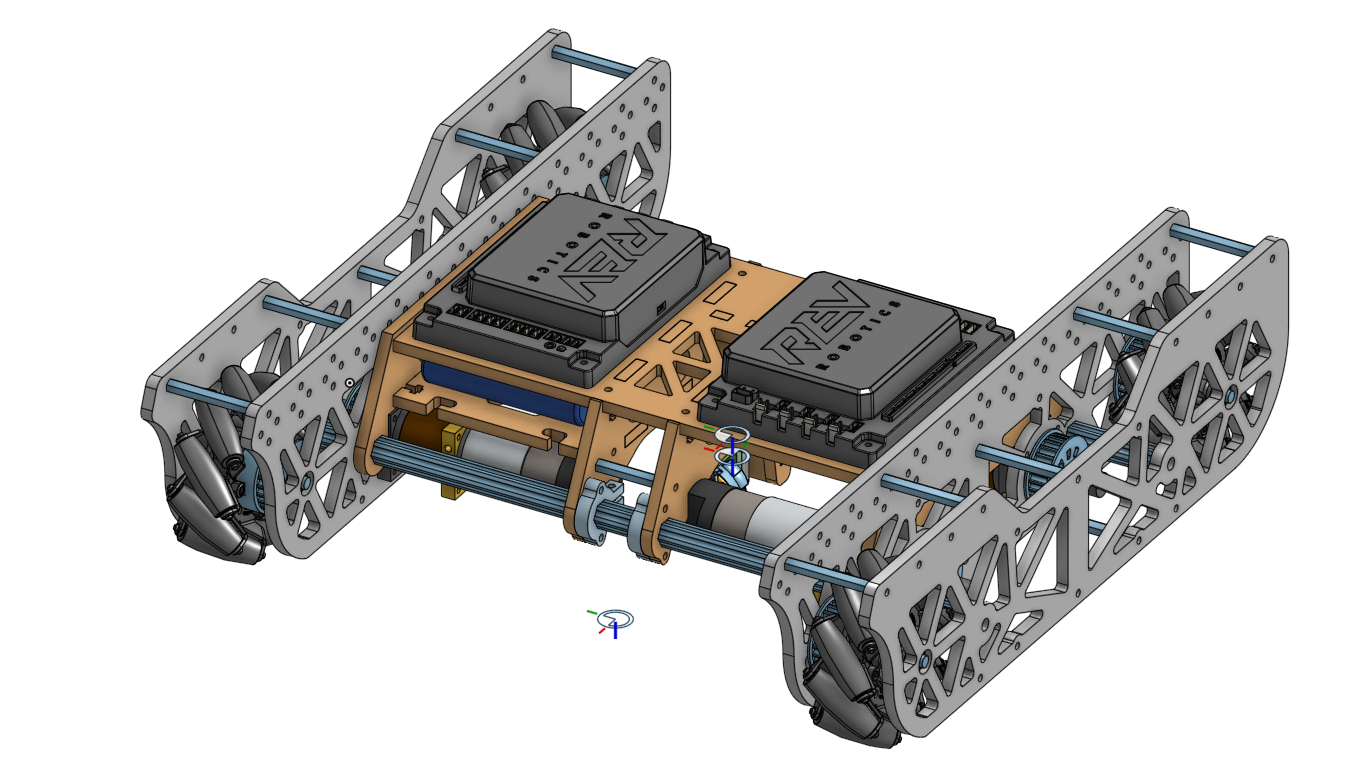
\includegraphics[width=0.9\textwidth, angle=0]{Meetings/August/08-08-21/8-8-21_Image6-FullAsm - Nathan Forrer.PNG}
\caption{This is our full assembly of the new drivetrain}
\label{fig:pic6}
\end{figure}